\documentclass[xcolor={dvipsnames},10pt]{beamer}
\definecolor{mypurple}{rgb}{0,0,98}

%---------------- Layout --------------------

\usecolortheme[named=mypurple]{structure} 
\usetheme[width=.15\paperwidth]{Hannover} 
\setbeamertemplate{items}[ball] 
\setbeamertemplate{blocks}[rounded][shadow=true]   %Problem with this template!!!!!!
\setbeamertemplate{footline}[frame number]
\setbeamertemplate{navigation symbols}{}

%----------------packages-------------------------------------


\usepackage[english]{babel} %for language support (ˆ enlever pour Žcrire en fran?ais)
\usepackage{amsmath,amsthm,amssymb ,euscript} % standard mathematics
\usepackage{rotating}        % handy packages
\usepackage{natbib}     % bibliography
\usepackage{geometry} % see geometry.pdf on how to lay out the page. There's lots.
\usepackage{graphicx}
%\usepackage{tabularx}



%%%%%%%%%%%%%%%%%%%%%%%%%%%%%%



%------------------------------------------------------------


\title[Formalising frieze patterns]{Formalising frieze patterns in Lean 4}
%\author{Antoine de Saint Germain}
\institute{The University of Hong Kong}
\date{30 August 2024}              


%------------------------------------------------------


 
\begin{document}

% Creates title page of slide show using above information
\begin{frame}
  \titlepage
\end{frame}


\begin{frame}
  \tableofcontents
\end{frame}

\section{Our project}
\begin{frame}



\end{frame}

\subsection{What is formalisation}
\begin{frame}


\end{frame}

\subsection{What is Lean 4}
\begin{frame}

\end{frame}

\subsection{Project outline}
\begin{frame}

\end{frame}


\section{Part 1: frieze patterns}
\subsection{Definitions}
\begin{frame}
\frametitle{Definitions}
{\bf Frieze pattern of height $n$}: map $f : \{0,1,\ldots , n,n+1\} \times \mathbb{Z} \longrightarrow \mathbb{Z}_{>0}$ with: \pause
 \begin{itemize}
 	\item Border of zeros:  $ f(0,m) = f (n+1,m) = 0, \quad \forall m \in \mathbb{Z}$, \pause
        \item Border of ones: $ f(1,m) = f (n,m) = 1, \quad \forall m \in \mathbb{Z}$, \pause
        \item  Diamond rule: $\forall (i,m) \in \{1,2,\ldots , n\} \times \mathbb{Z}$,
       \[
            f(i,m) f(i,m+1) = 1 + f(i+1,m) f(i-1, m+1). \pause
        \]
 \end{itemize}
 \begin{figure}
 	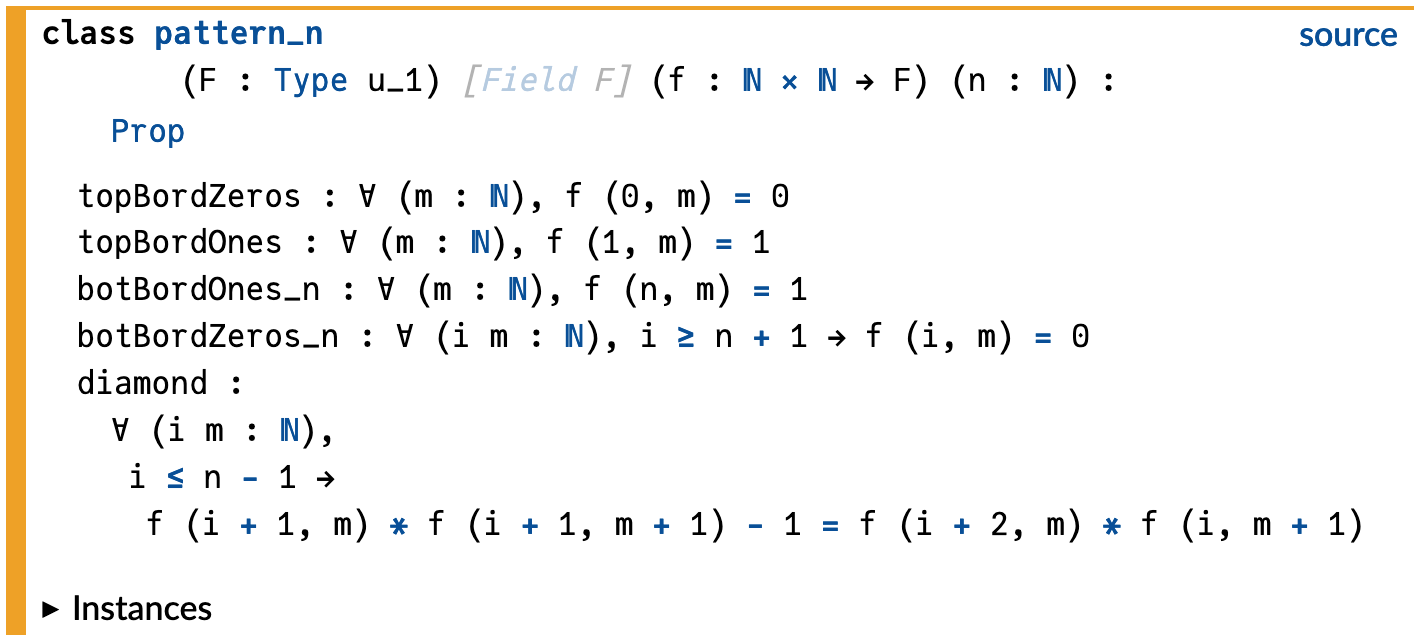
\includegraphics[width = \textwidth]{pic1}
 \end{figure}
\end{frame}

\begin{frame}
\frametitle{Definitions}
\begin{figure}
	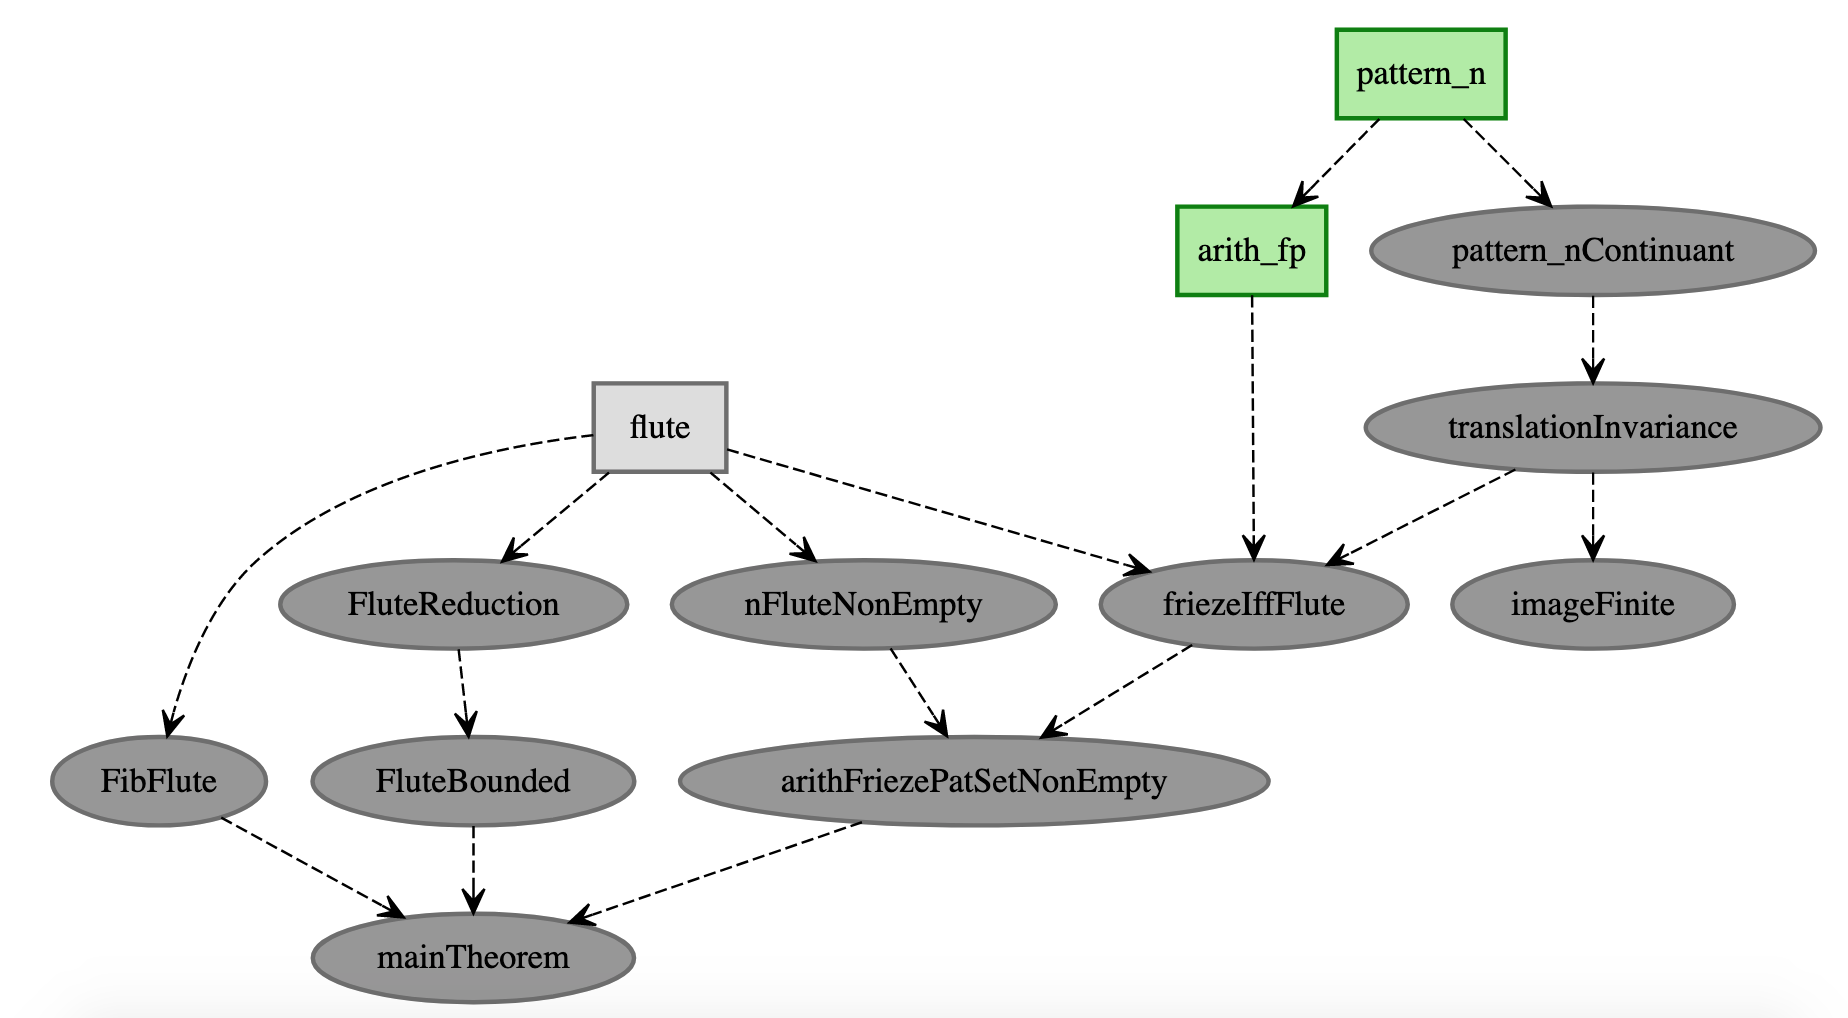
\includegraphics[width=\textwidth]{pic2}
\end{figure}
\end{frame}


\subsection{Translation-invariance}
\begin{frame}
\frametitle{Translation invariance}
{\bf Proposition.} (Coxeter, 1971) Frieze patterns of height $n$ are $(n+1)$-periodic. \pause
\begin{figure}
	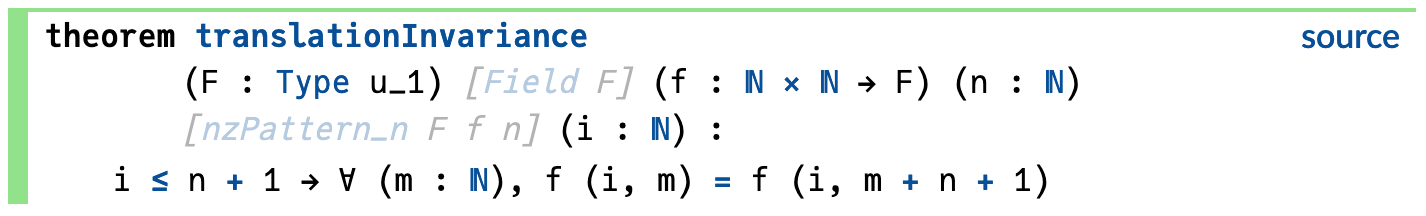
\includegraphics[width=\textwidth]{pic3}
\end{figure}
\end{frame}


\begin{frame}
\frametitle{Translation invariance}
\begin{figure}
	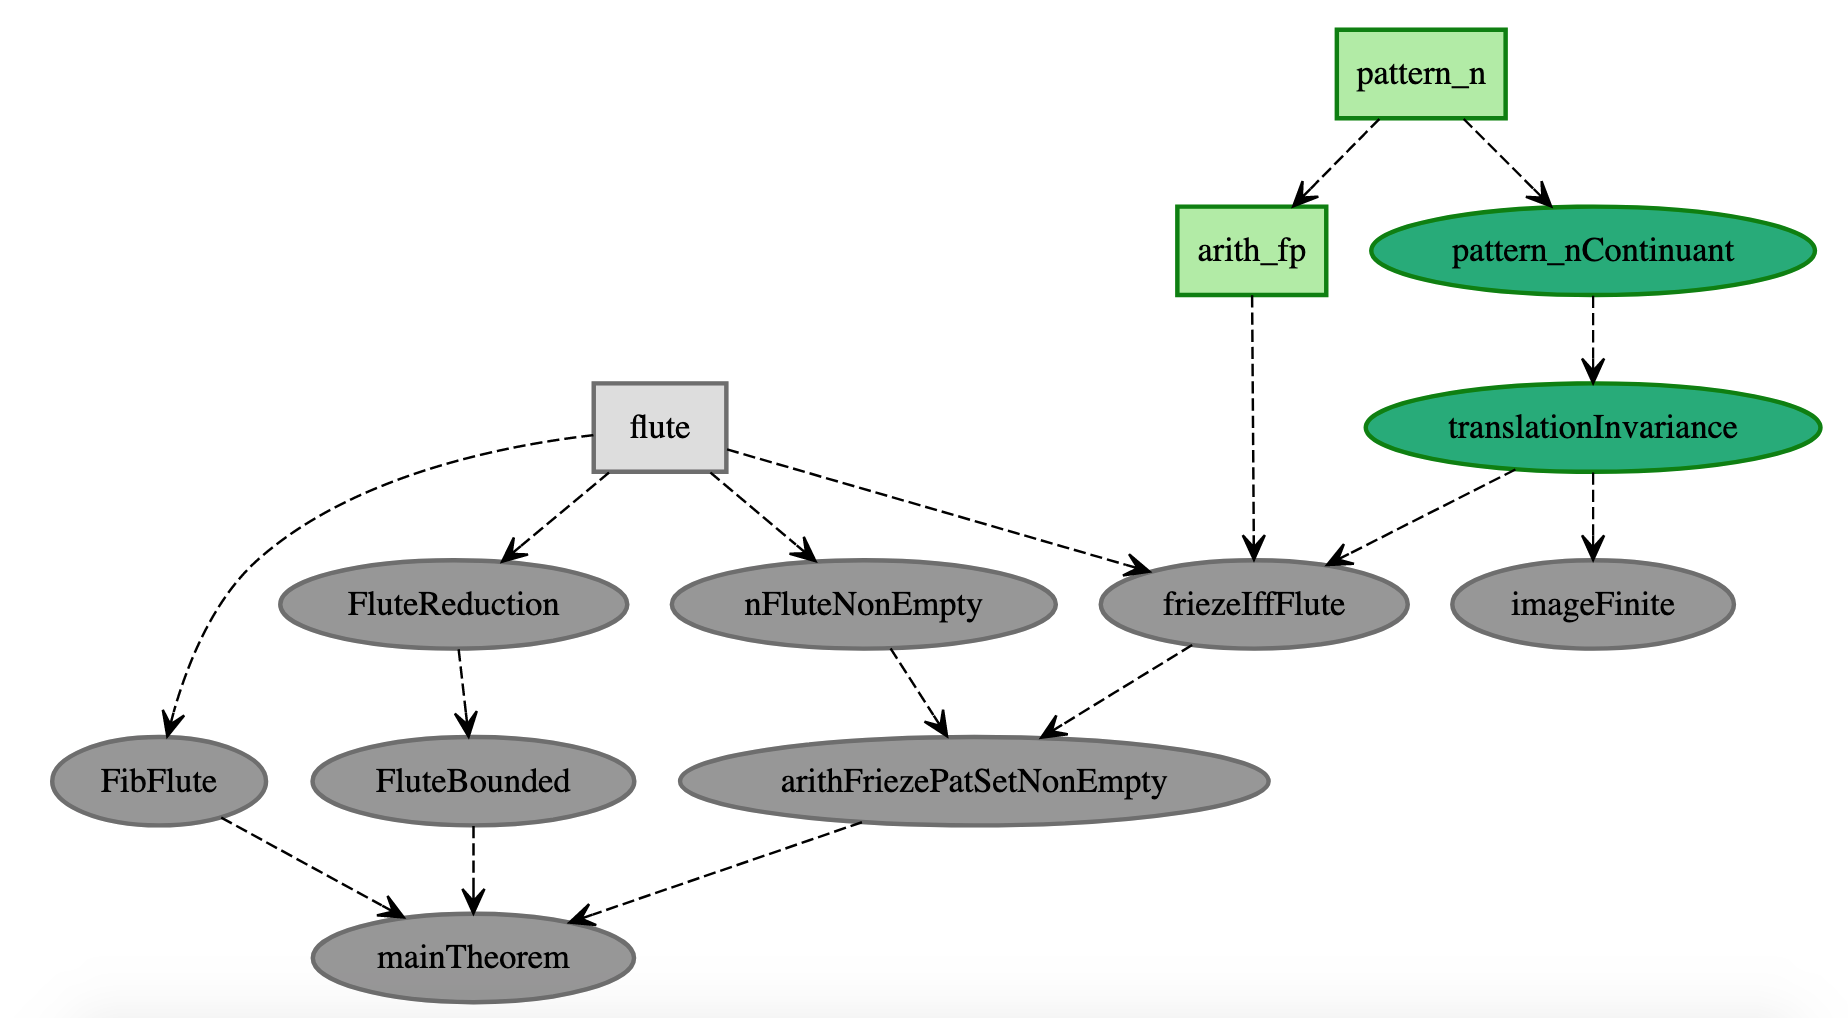
\includegraphics[width=\textwidth]{pic4}
\end{figure}
\end{frame}


\section{Part 2: Pandean flutes}
\subsection{Definitions}
\begin{frame}
\frametitle{Definitions}
{\bf Pan flute of height $n$}: $n$-tuple of {\it positive integers} $(a_1, \ldots, a_n)$ such that \pause
\begin{itemize}
	\item $a_1 = 1$, \pause
	\item $a_n = 1$, \pause
	\item $a_i \mid (a_{i-1}+ a_{i+1}), \quad \forall i \in \{2,\ldots, n-1\}$.
\end{itemize}
\begin{figure}
	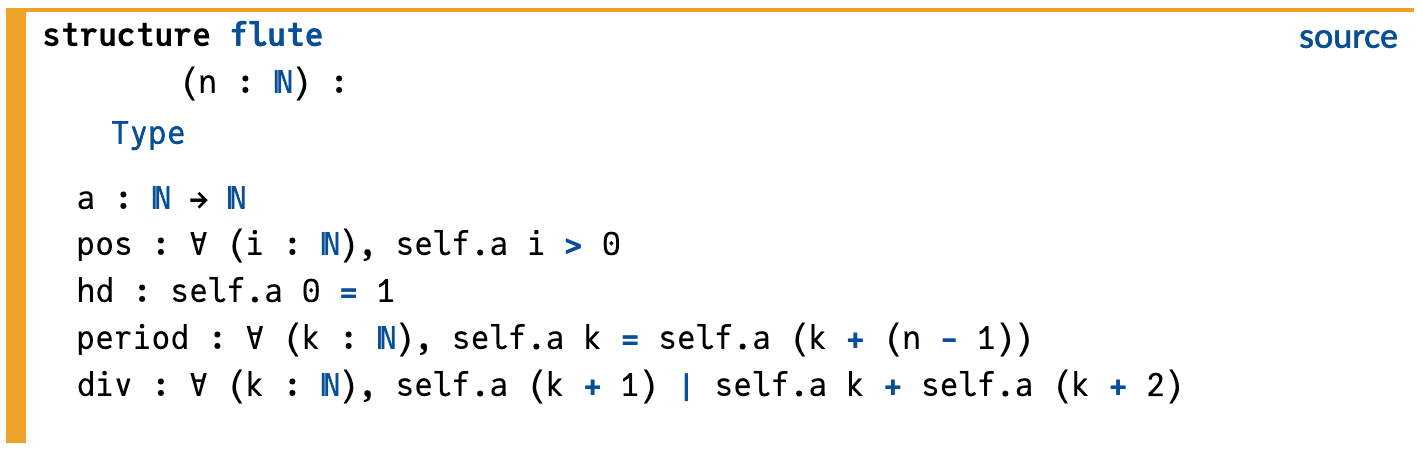
\includegraphics[width=\textwidth]{pic5}
\end{figure}
\end{frame}

\begin{frame}
\frametitle{Definitions}
\begin{figure}
	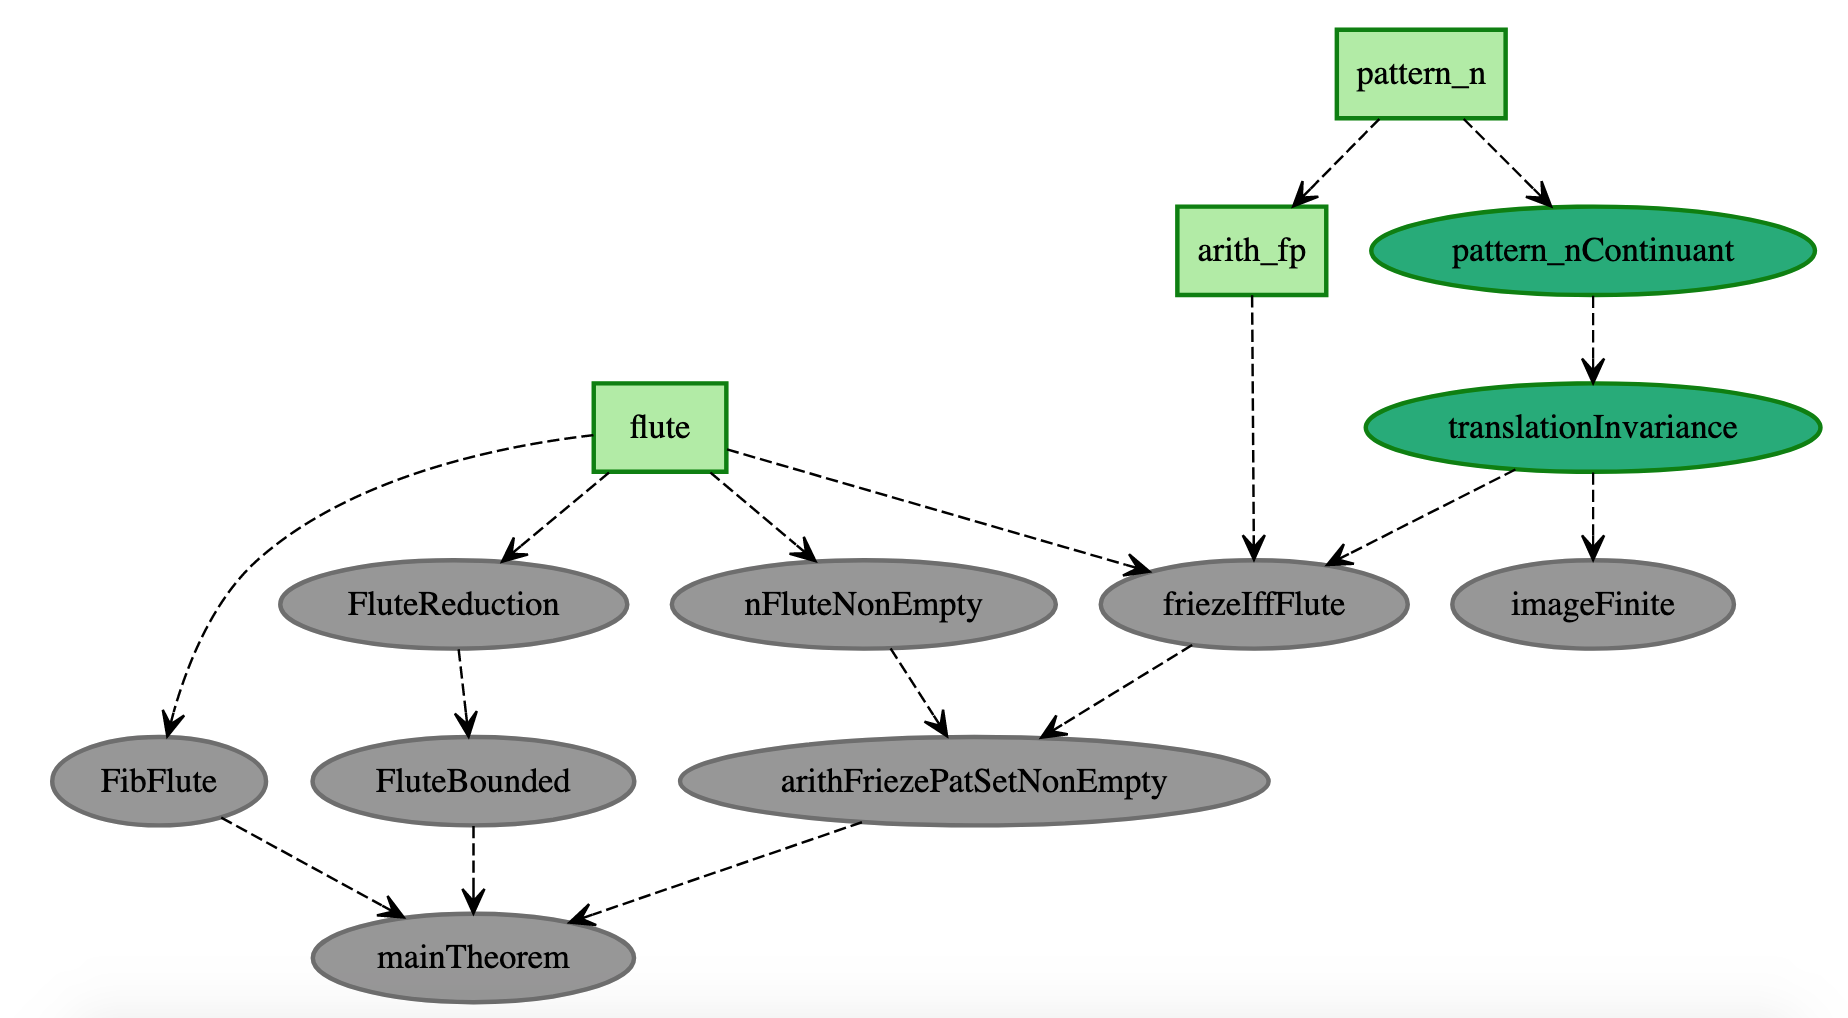
\includegraphics[width=\textwidth]{pic6}
\end{figure}
\end{frame}


\subsection{Upper bounds on flutes}
\begin{frame}
\frametitle{Upper bounds on flutes}
Fibonacci sequence: 
\begin{itemize}
	\item[Base.] $F_0 = 0, F_1 = 1, $\pause
	\item[IH.] $\forall n \geq 0, F_{n+2} = F_{n+1} + F_n. $ \pause
\end{itemize}
{\bf Proposition.} \pause For any flute $(a_1, \ldots , a_n)$ of height $n$, we have
\[
	a_i \leq F_n. \pause
\]
\begin{figure}
	
\includegraphics[width=\textwidth]{pic7}
\end{figure}
\end{frame}



\begin{frame}
\frametitle{Upper bounds on flutes}
\begin{figure}
	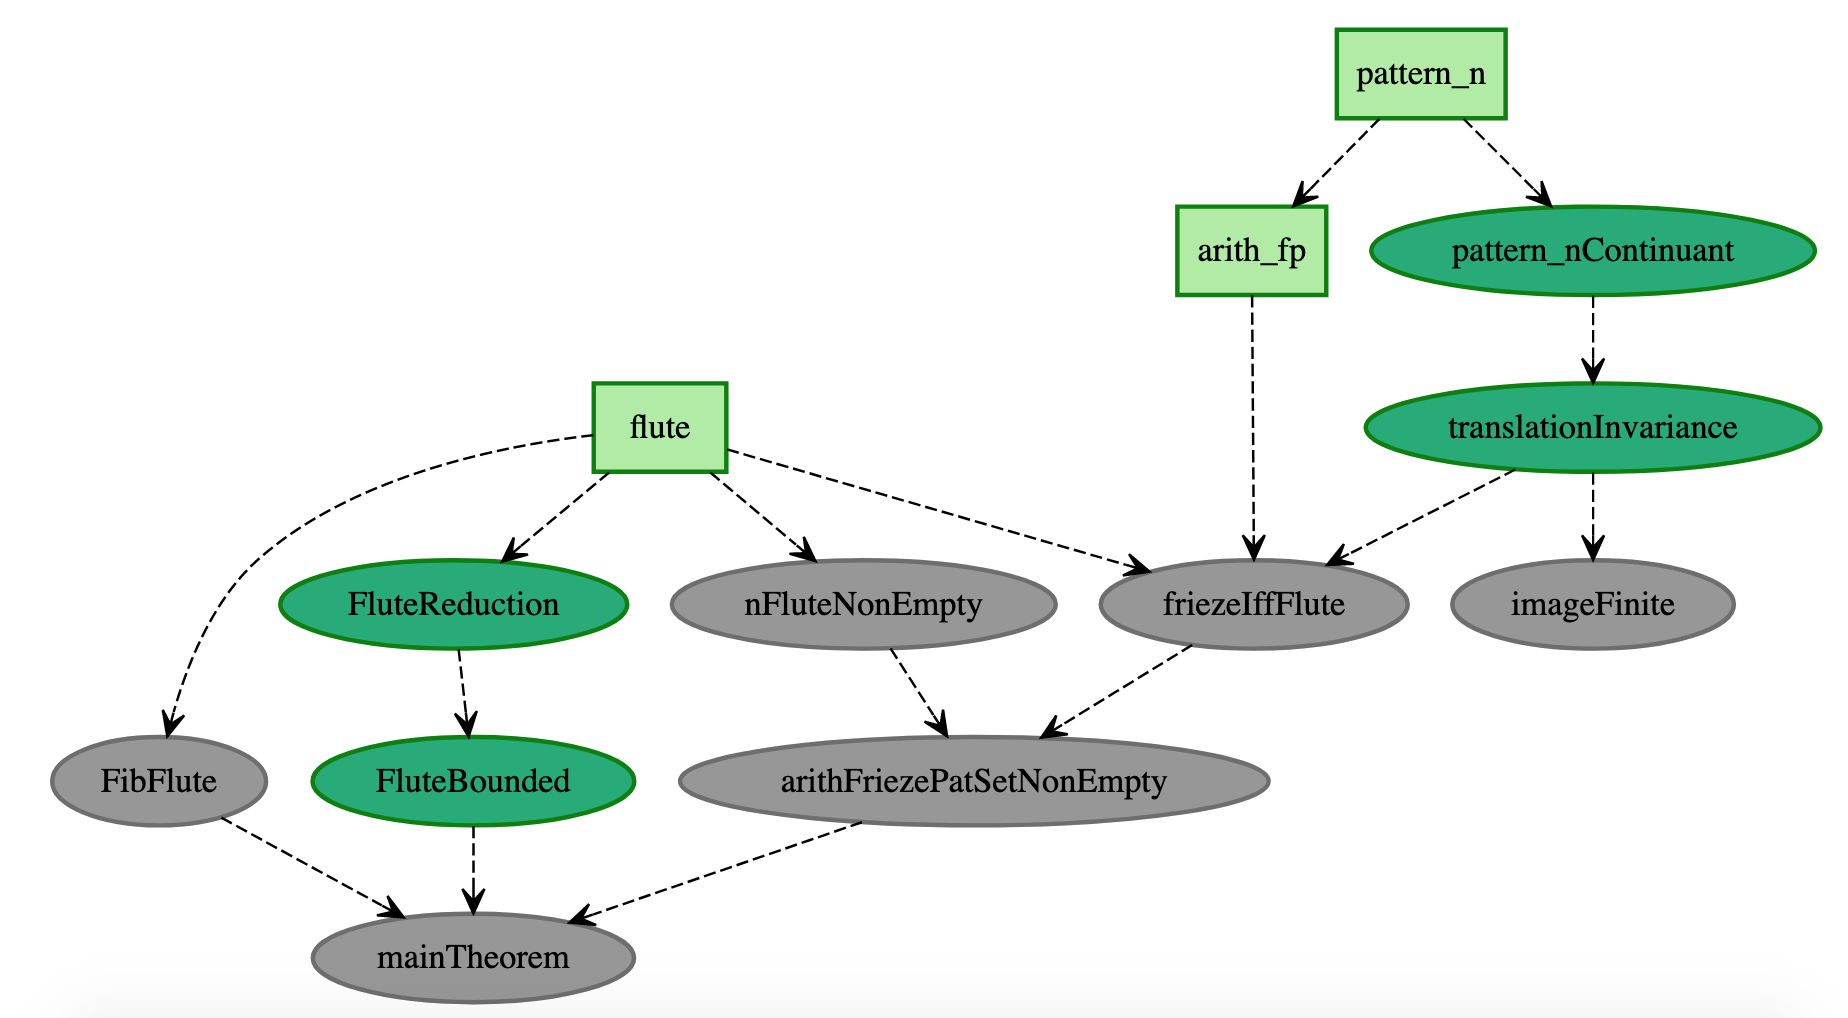
\includegraphics[width=\textwidth]{pic8}
\end{figure}
\end{frame}

\subsection{Fibonacci flutes}
\begin{frame}
\frametitle{Fibonacci flutes}
{\bf Proposition.} There exists a flute $(f_1, \ldots, f_n)$ of height $n$ such that 
\[
	f_i = F_n, \quad \text{for some}\;  i \in \{1, \ldots, n\}. \pause
\]	

{\bf Proof.} By construction. \pause When $n$ is even, take
\[
	(F_1, F_3, \ldots, F_{n-1}, F_n, F_{n-2}, \ldots, F_4,F_2). \pause
\]
When $n$ is odd, take 
\[
	(F_1, F_3, \ldots, F_{n-2}, F_n, F_{n-1}, \ldots, F_4,F_2). \pause
\]
\begin{figure}
	%\includegraphics[width=\textwidth]{pic9}
	% Might not be very interesting to add the Lean code for this one ?
\end{figure}
\end{frame}



\begin{frame}
\frametitle{Fibonacci flutes}
\begin{figure}
	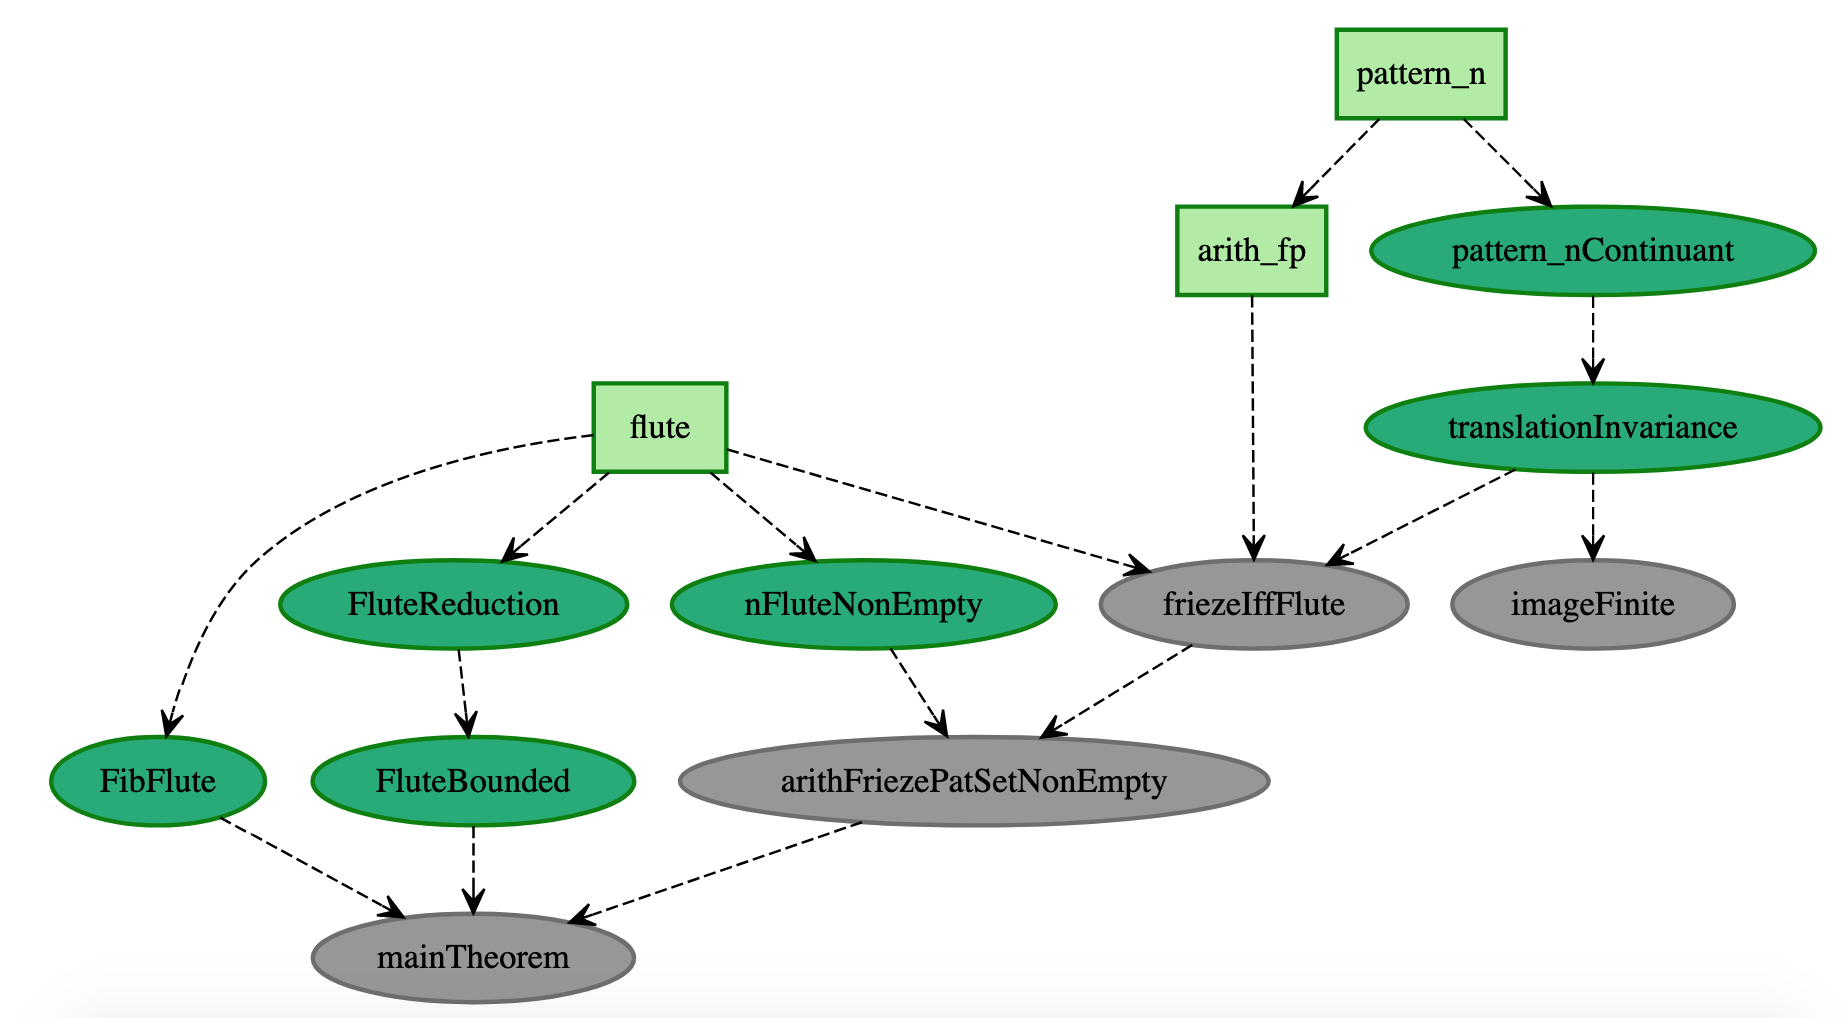
\includegraphics[width=\textwidth]{pic10}
\end{figure}
\end{frame}



\section{Part 3: Proving the main result}
\subsection{Flutes and friezes}
\begin{frame}
\frametitle{Friezes consist of flutes}
{\bf Proposition.} Let $f$ be a frieze pattern of height $n$. \pause For all $m \in \mathbb{Z}$,
\[
	(f (1,m), f(2,m), \ldots, f (n-1,m), f(n,m) )
\]
is a flute of height $n$. \pause
\begin{figure}
	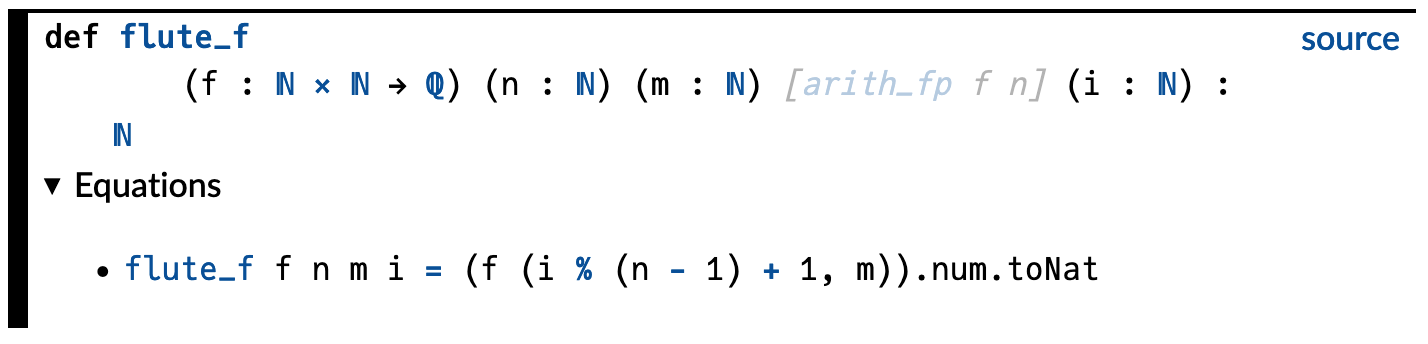
\includegraphics[width=\textwidth]{pic11}
\end{figure}

\end{frame}


\begin{frame}
\frametitle{Flutes give rise to friezes}
{\bf Proposition.} Let $f = (f_1, \ldots, f_n)$ be a flute of height $n$. \pause 
There exists a (unique) frieze pattern $\mathcal{F}$ of height $n$ with
\[
	\mathcal{F}\vert_{m=0} = (0, f_1, f_2, \ldots, f_{n-1}, f_n, 0).\pause
\]
\begin{figure}
	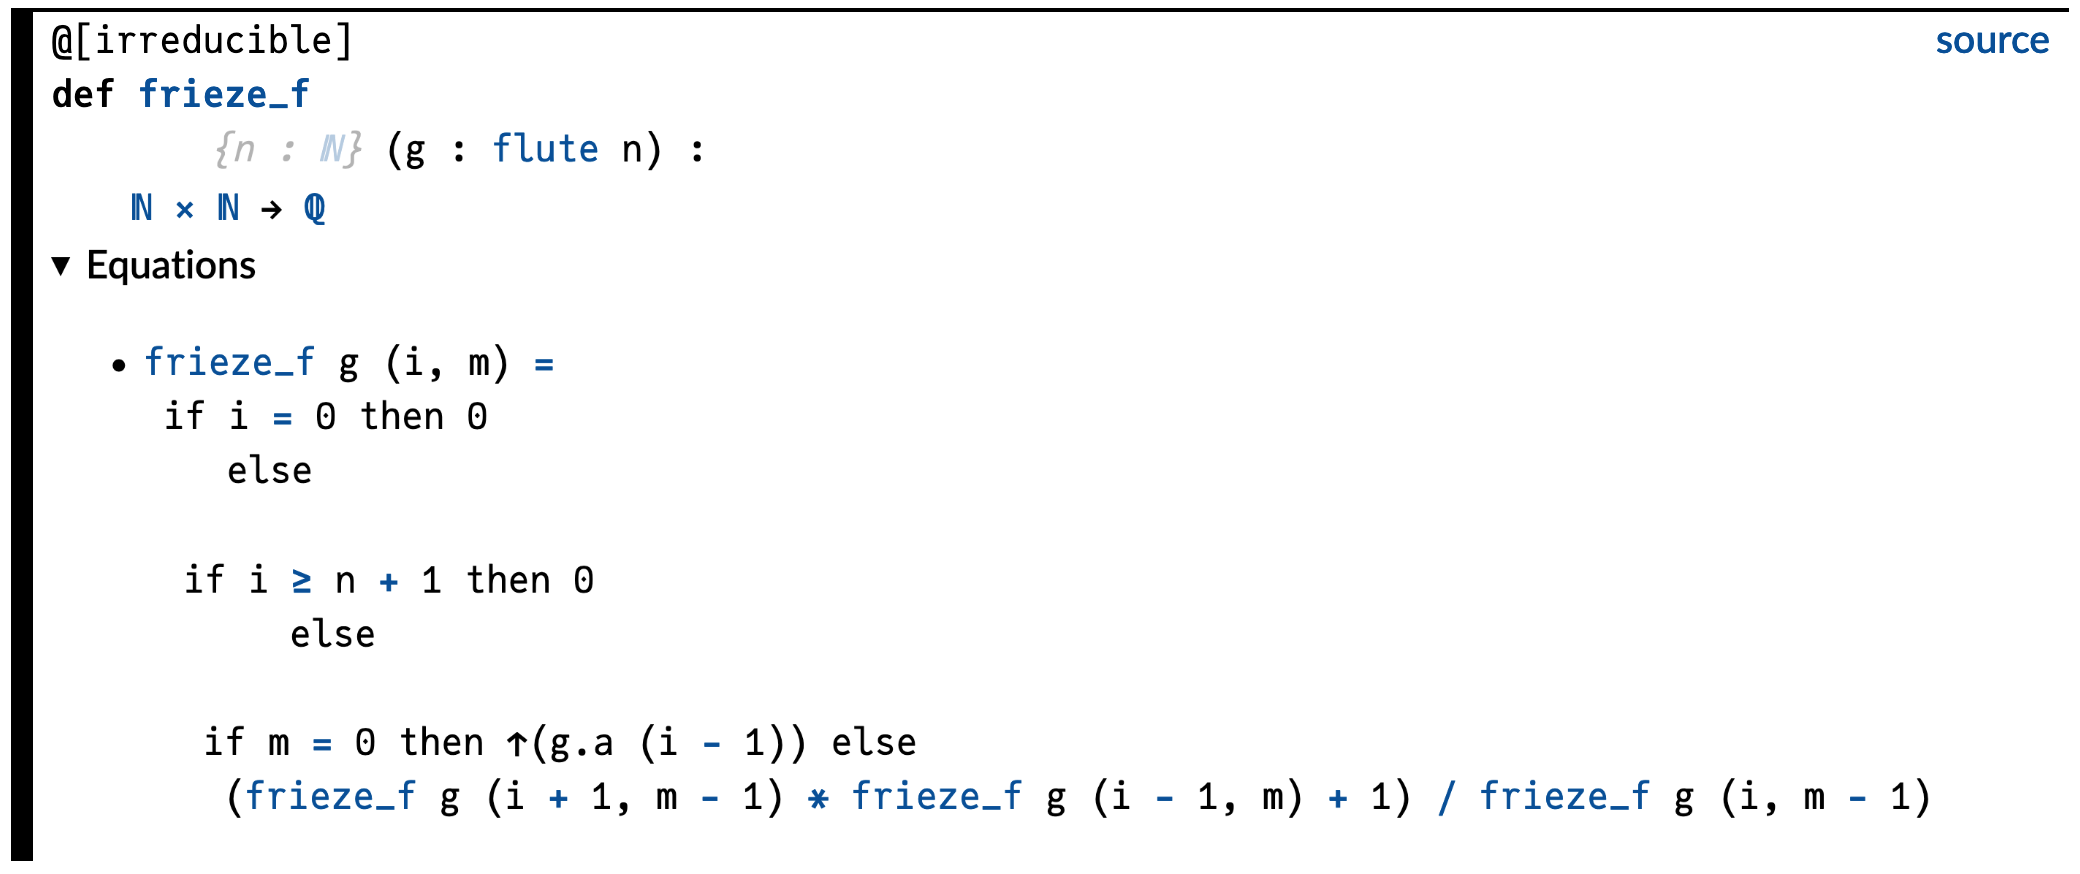
\includegraphics[width=\textwidth]{pic12}
\end{figure}
\end{frame}

\begin{frame}
\frametitle{Flutes give rise to friezes}
\begin{figure}
	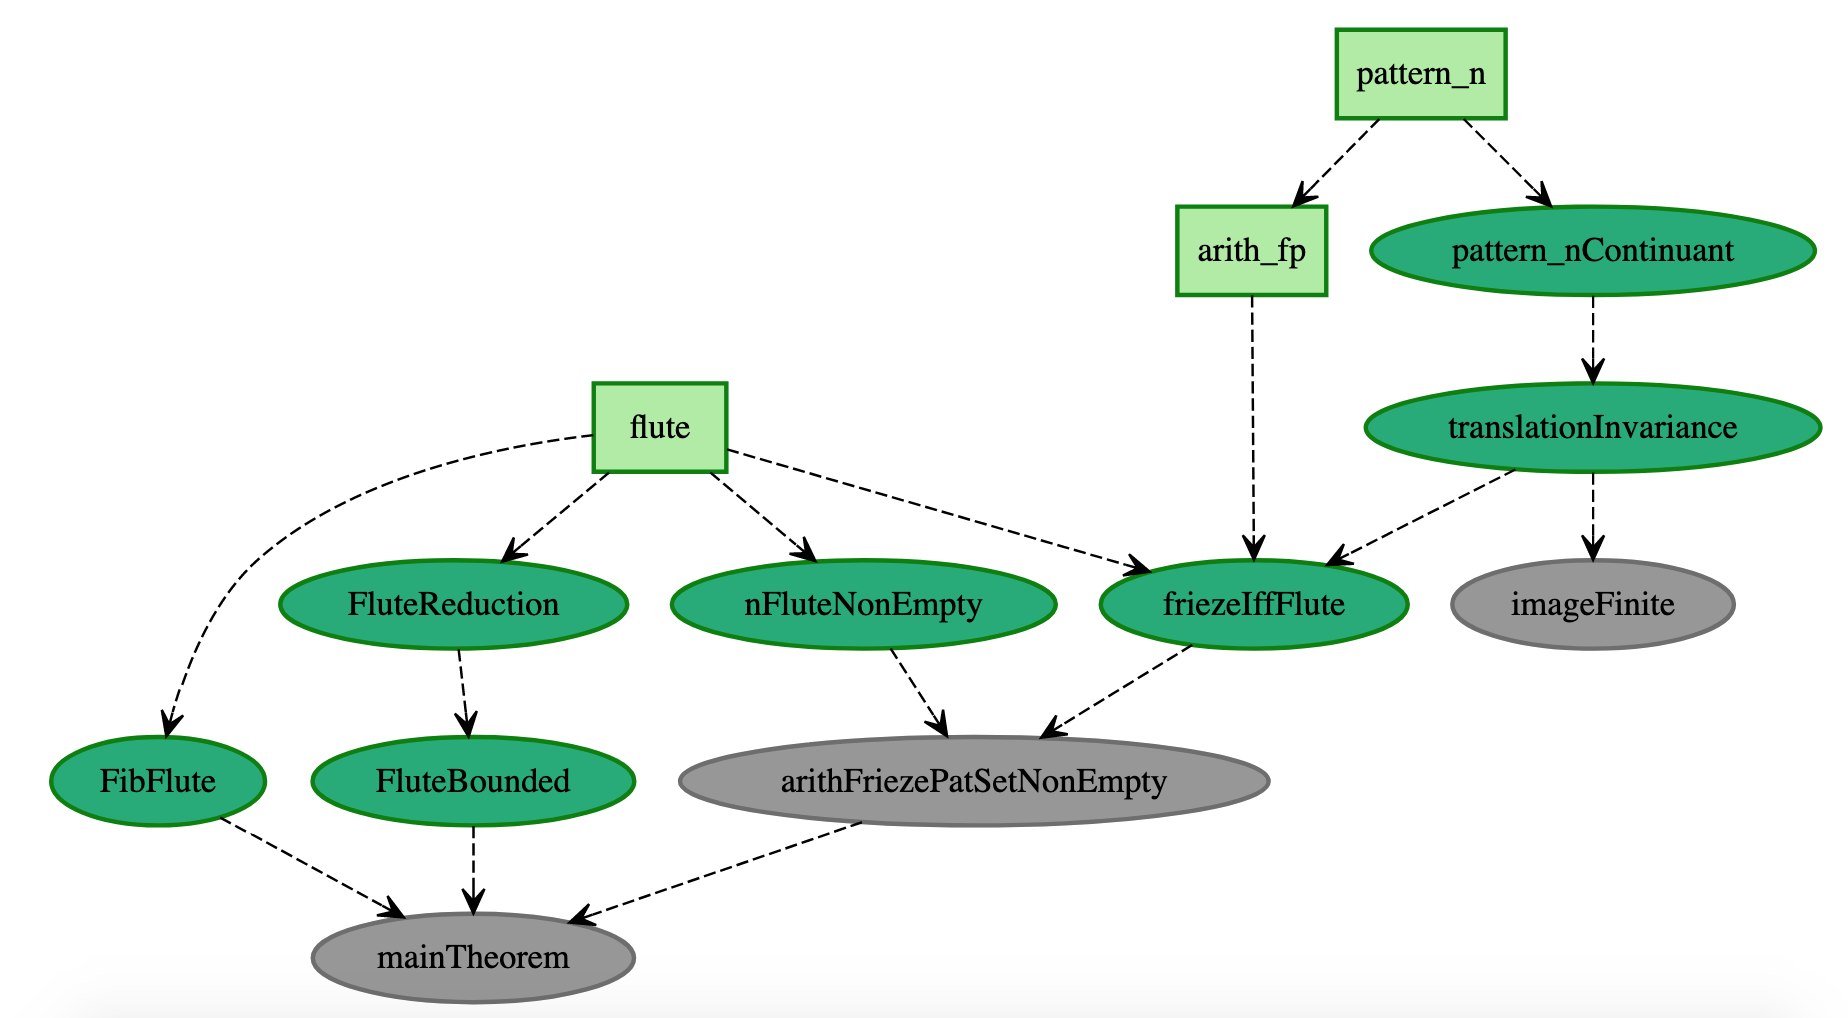
\includegraphics[width=\textwidth]{pic13}
\end{figure}
\end{frame}

\subsection{Main theorem}
\begin{frame}
\frametitle{Main theorem}
$u_n := \max (f (i,m) : \forall i , \forall m , \forall \text{ frieze patterns } $f$ \text{ of height }n).$ \pause
{\bf Theorem.} We have 
\[
	u_n = F_n, \quad \forall n \geq 1. \pause
\]
\begin{figure}
	
\includegraphics[width=\textwidth]{pic14}
\end{figure}
\end{frame}

\begin{frame}
\frametitle{Main theorem}
\href{https://antoine-dsg.github.io/frieze_patterns/blueprint/}{Project complete !}
\end{frame}




\end{document}

